\documentclass[border=4pt]{standalone}
\usepackage{tikz}
\usetikzlibrary{decorations.pathmorphing,arrows.meta}
\begin{document}
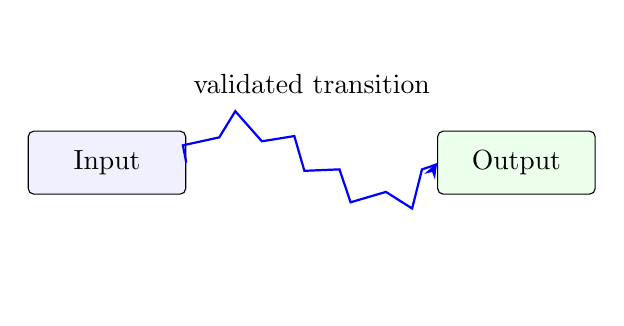
\begin{tikzpicture}[
  stage/.style={draw,rounded corners=2pt,minimum width=20mm,minimum height=8mm,fill=blue!6},
  signal/.style={-{Stealth[length=2mm]},line width=.8pt,blue}
]
  \node[stage] (input) at (-2.6,0) {Input};
  \node[stage,fill=green!8] (output) at (2.6,0) {Output};
  \draw[signal,decorate,decoration={zigzag,segment length=7mm,amplitude=1.4mm}]
    (input.east) .. controls (-.7,1.7) and (.7,-1.7) .. (output.west);
  \node[above] at (0,.75) {validated transition};
\end{tikzpicture}
\end{document}
